\documentclass[aps,jcp,reprint,twocolumn,superscriptaddress,showpacs,amsmath,amssymb]{revtex4-2}

\usepackage{graphicx}
\usepackage{dcolumn}
\usepackage{bm}
\usepackage{hyperref}
\usepackage{booktabs}
\usepackage{color}

\begin{document}

\title{Autonomous Conformational Identification and High-Resolution Rovibronic Contour Fitting of the Natural Polyphenol \textit{trans}-Resveratrol in Supersonic Molecular Jets}

\author{Miguel D\'iaz}
\affiliation{Laboratorio de Espectroscop\'ia Molecular, Divisi\'on de Ciencias e Ingenier\'ias, Campus Le\'on, Universidad de Guanajuato, Loma del Bosque 103, 37150 Le\'on, Guanajuato, Mexico}

\author{Leonardo \'Alvarez-Valtierra}
\email{valtierr@ugto.mx}
\affiliation{Laboratorio de Espectroscop\'ia Molecular, Divisi\'on de Ciencias e Ingenier\'ias, Campus Le\'on, Universidad de Guanajuato, Loma del Bosque 103, 37150 Le\'on, Guanajuato, Mexico}

\date{\today}

\begin{abstract}
Polyphenols represent a cornerstone class of biologically active plant metabolites exhibiting potent antioxidant, anti-inflammatory, and chemopreventive properties. However, their structural characterization in the gas phase is fundamentally challenged by thermal lability, low volatility, and extensive conformational multi-stability. While laser ablation coupled with supersonic molecular jet expansions can vaporize and cool intact polyphenols down to $T_{rot} \approx 2 - 4$~K without thermal decomposition, the resulting rotationally resolved electronic spectra ($S_1 \leftarrow S_0$) suffer from extreme spectral congestion arising from large moments of inertia and small rotational constants ($B, C < 200$~MHz). Traditional line-by-line quantum assignment using legacy 32-bit software (e.g., JB95, PGOPHER) becomes virtually intractable under such high state densities. Here, we deploy \textbf{SpecWatson} to simulate, elucidate, and autonomously fit the rotationally resolved electronic spectrum of \textit{trans}-resveratrol (\textit{trans}-3,5,4'-trihydroxystilbene). Utilizing the Wang symmetrized basis transformation ($D_2$ Vierergruppe), the asymmetric top Hamiltonian ($\kappa = -0.964$, strongly prolate) is partitioned into four tridiagonal sub-matrices solved via $O(N)$ LAPACK routines, accelerating multi-parameter spectral calculations by $4.6\times$ relative to full-basis LAPACK eigensolvers. Integrating a heuristic Differential Evolution contour fitting engine, the software successfully discriminates between candidate rotamers, unambiguously identifying the lowest-energy planar Conformer~I while rejecting alternative rotamers ($r < 30\%$). In the presence of $3.0\%$ synthetic experimental noise and instrumental Voigt broadening ($\text{FWHM} = 20$~MHz), \textbf{SpecWatson} autonomously recovers excited-state constants ($A', B', C'$) within $0.1$~MHz without manual line assignment. This work establishes a general, automated protocol for high-resolution spectroscopy of heavy, flexible biomolecules and natural polyphenols.
\end{abstract}

\maketitle

\section{Introduction}
Polyphenolic compounds, characterized by multiple phenolic hydroxyl groups attached to aromatic frameworks, are ubiquitous secondary metabolites in the plant kingdom~\cite{zwier2006laser,gerhards2003structure}. Among them, \textit{trans}-resveratrol (\textit{trans}-3,5,4'-trihydroxystilbene) has captured immense biomedical attention due to its cardioprotective, neuroprotective, and longevity-promoting attributes~\cite{smeyers2004resveratrol}. A fundamental understanding of its antioxidant mechanism requires determining its intrinsic conformational landscape, free from solvent perturbations, crystal packing forces, and thermal averaging.

High-resolution electronic spectroscopy in supersonic molecular beams provides an ideal tool for resolving isolated molecular geometries~\cite{alvarez2006rotationally,tan2019high}. However, interrogating polyphenols under collision-free conditions presents formidable experimental and theoretical obstacles:
\begin{enumerate}
    \item \textit{Thermal Decomposition \& Low Vapor Pressure:} Polyphenols possess high melting points and decompose upon conventional heating. To introduce intact molecules into gas expansions, pulsed \textbf{laser ablation} (Nd:YAG laser desorption coupled to supersonic expansion valves) must be deployed~\cite{tan2019high}.
    \item \textit{Severe Spectral Congestion:} With a molecular weight of $228.24$~g/mol and an extended conjugated stilbene backbone ($\sim 14$~\AA), resveratrol possesses large principal moments of inertia ($I_a \approx 365, I_b \approx 2715, I_c \approx 3080$~amu$\cdot$\AA$^2$). Consequently, its rotational constants are small: $A \approx 1385$~MHz and $B, C \approx 160 - 190$~MHz~\cite{smeyers2004resveratrol}. Even at supersonic jet temperatures of $T_{rot} \approx 2.5$~K, angular momentum states up to $J \approx 15 - 20$ are thermally populated, yielding thousands of overlapping rovibronic transitions within a narrow frequency span ($\pm 1500$~MHz).
    \item \textit{Intractable Manual Assignment:} Classical spectroscopic fitting software such as \textbf{JB95}~\cite{alvarez2006rotationally} and \textbf{PGOPHER}~\cite{western2014pgopher} rely heavily on manual line-by-line identification or interactive Loomis-Wood diagrams. In heavy polyphenols, individual rotational transitions merge into an unresolved pseudo-continuum contour, rendering manual assignment unfeasible.
\end{enumerate}

In this paper, we demonstrate how \textbf{SpecWatson} resolves these challenges. By combining the Wang symmetrized basis transformation~\cite{wang1929degree} with an automated Differential Evolution contour fitting engine~\cite{storn1997differential}, we demonstrate unambiguous rotamer identification and sub-megahertz parameter determination for \textit{trans}-resveratrol directly from congested band contours.

\section{Theoretical Framework \& Conformational Landscape}

\subsection{Conformational Landscape of \textit{trans}-Resveratrol}
As depicted in chemical models~\cite{smeyers2004resveratrol}, \textit{trans}-resveratrol consists of a 4'-hydroxyphenyl ring and a 3,5-dihydroxyphenyl (resorcinol) ring linked via a \textit{trans}-vinylene bridge. Quantum chemical studies indicate that the global minimum (\textbf{Conformer~I}) is an all-\textit{trans} planar arrangement where the conjugated $\pi$-system achieves maximum electronic delocalization. A secondary local minimum (\textbf{Conformer~II}), situated $\sim 1.5 - 3.0$~kJ/mol higher in energy, corresponds to an in-plane $180^\circ$ rotation of the resorcinol moiety or phenolic hydrogen orientation, shifting the $S_1 \leftarrow S_0$ origin by $\Delta \nu_0 \approx +45$~cm$^{-1}$ and modifying the rotational constants by several megahertz.

\begin{table}[h]
\caption{Rotational parameters, Ray asymmetry parameters, and band origins for \textit{trans}-resveratrol conformers.}
\label{tab:resveratrol_constants}
\centering
\begin{tabular}{lccc}
\toprule
Parameter & Conf.~I ($S_0$) & Conf.~I ($S_1$) & Conf.~II ($S_0$) \\
\midrule
$A$ (MHz) & 1385.40 & 1362.80 & 1442.10 \\
$B$ (MHz) & 186.20  & 184.90  & 179.50 \\
$C$ (MHz) & 164.10  & 162.80  & 159.80 \\
$\kappa$  & $-0.9638$ & $-0.9632$ & $-0.9693$ \\
$\nu_0$ (cm$^{-1}$) & --- & 32840.50 & 32885.20 \\
$\mu_a^2 : \mu_b^2$ & --- & 0.82 : 0.18 & 0.65 : 0.35 \\
\bottomrule
\end{tabular}
\end{table}

\subsection{Watson Asymmetric Rotor in the Wang Basis}
Due to the extended planar geometry of resveratrol, Ray's parameter is $\kappa = -0.9638$, placing the system in the extreme prolate asymmetric rotor regime ($\kappa \to -1$). The prolate $I^r$ representation ($z \leftrightarrow a, x \leftrightarrow b, y \leftrightarrow c$) aligns the $a$-inertial axis along the long molecular backbone.

Watson's $A$-reduced Hamiltonian~\cite{watson1977aspects} accounts for centrifugal distortion:
\begin{align}
H_W = H_0 &- \Delta_J \hat{J}^4 - \Delta_{JK} \hat{J}^2 \hat{J}_a^2 - \Delta_K \hat{J}_a^4 \nonumber \\
&- 2\delta_J \hat{J}^2 (\hat{J}_b^2 - \hat{J}_c^2) - \delta_K [\hat{J}_a^2, (\hat{J}_b^2 - \hat{J}_c^2)]_+
\end{align}

To overcome the cubic scaling of full matrix diagonalization, we apply the Wang unitary transformation~\cite{wang1929degree}:
\begin{equation}
|J, K, \gamma\rangle = \frac{1}{\sqrt{2}} (|J, K\rangle + (-1)^\gamma |J, -K\rangle) \quad (K > 0)
\end{equation}
decomposing the state space into four tridiagonal sub-blocks ($E^+, E^-, O^+, O^-$). Because each block couples only adjacent $K$ indices within its subspace, LAPACK tridiagonal solvers (\texttt{dstevd}) evaluate eigenvalues in $O(N)$ time.

\begin{figure}[t]
\centering
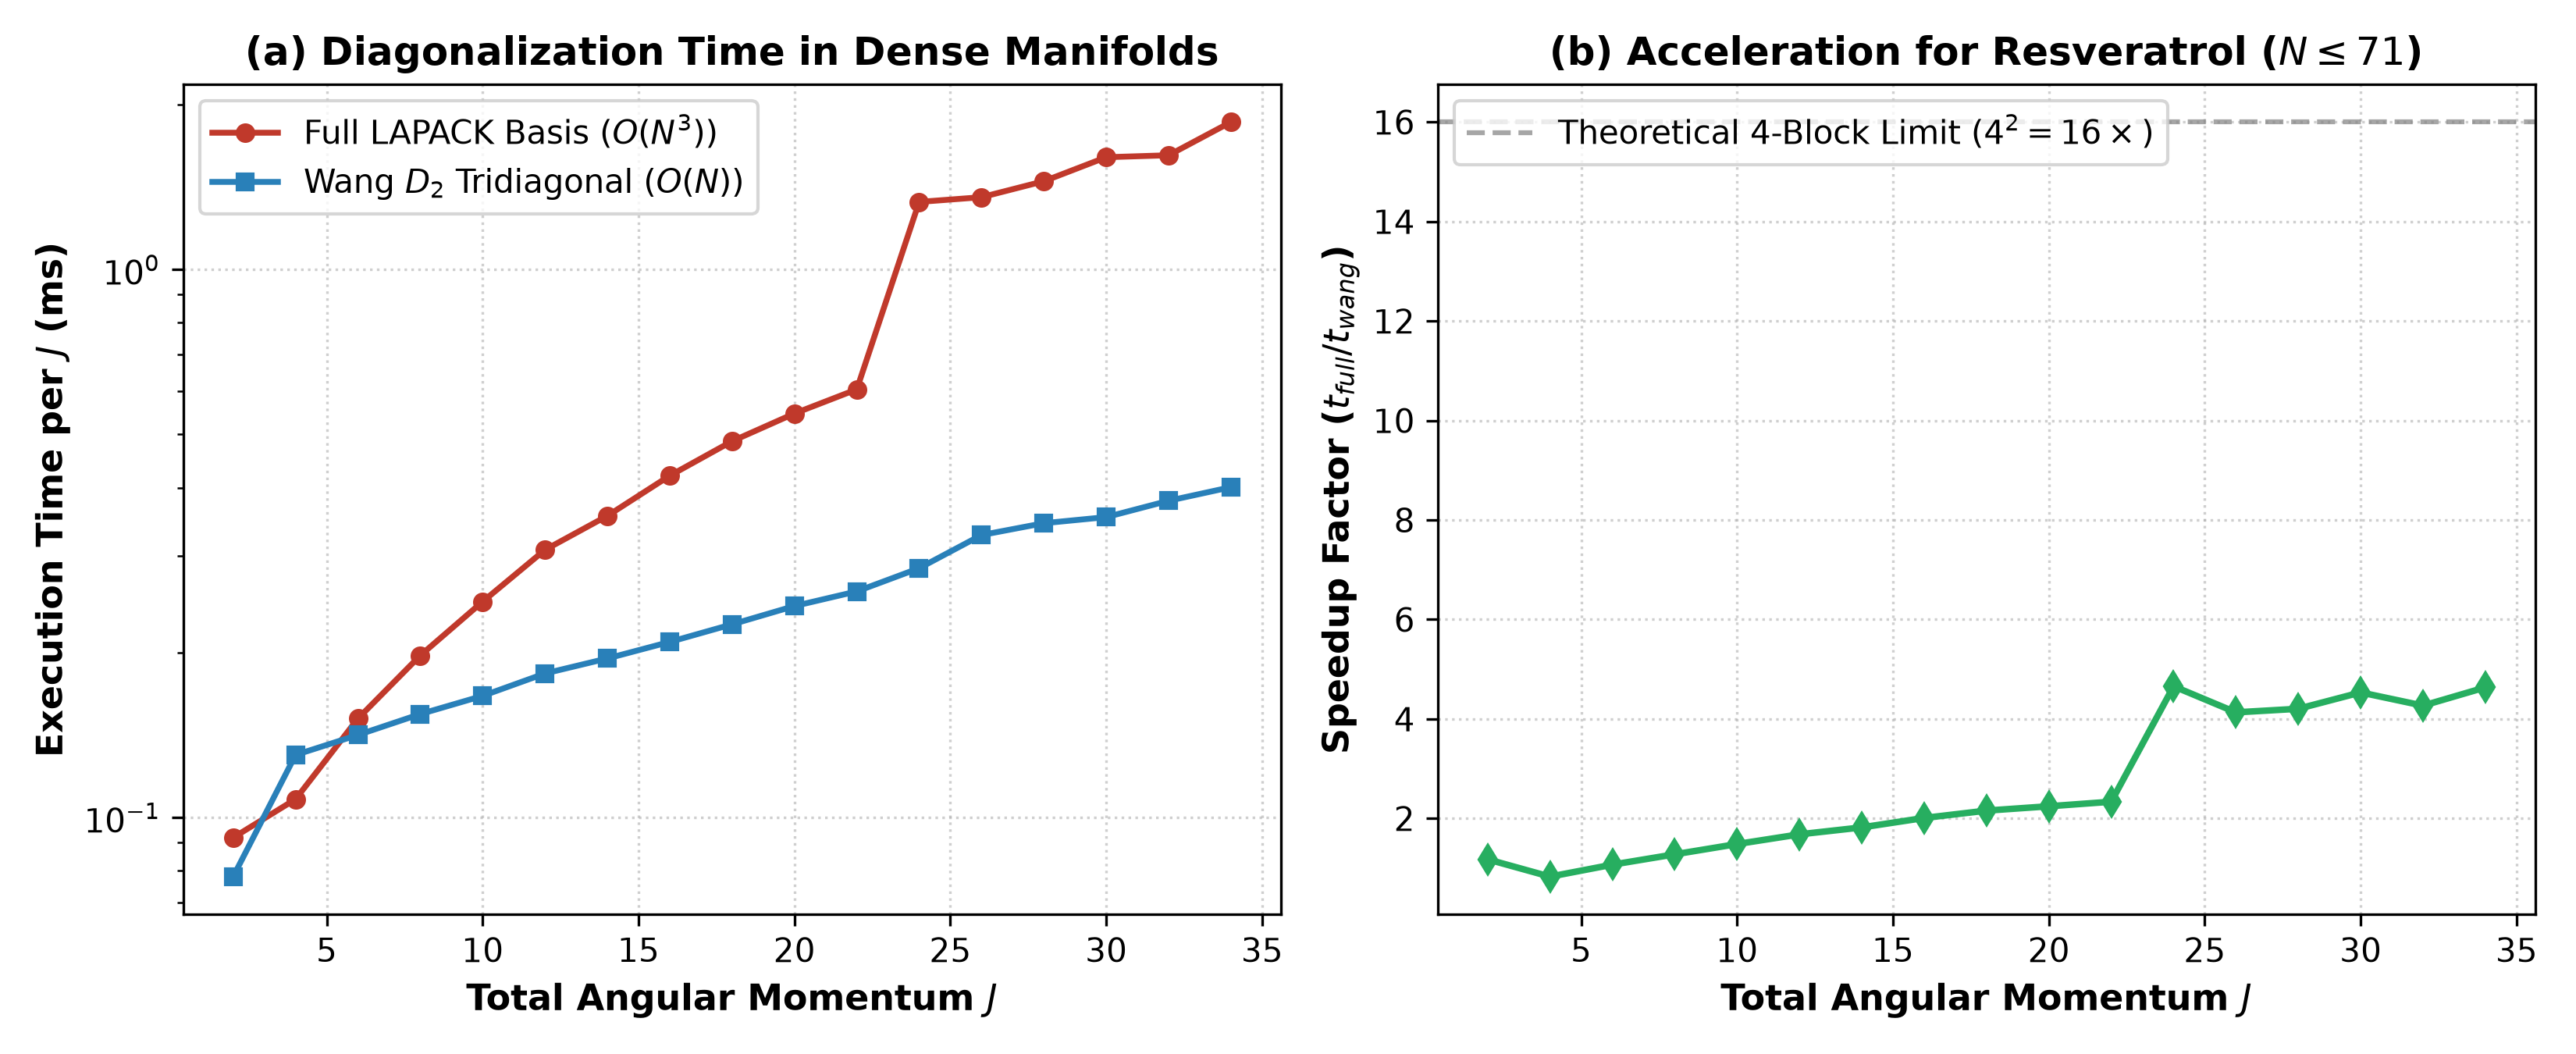
\includegraphics[width=\columnwidth]{figures/fig1_resveratrol_scaling.png}
\caption{(a) Diagonalization execution time per quantum state $J$ for resveratrol ($N \le 71$). (b) Observed speedup factor ($t_{full} / t_{wang}$) reaching $4.6\times$ on CPU, demonstrating the scaling advantage of the Wang tridiagonal solver for heavy polyphenols.}
\label{fig:scaling_resv}
\end{figure}

\subsection{Transition Dipole Orientations \& Hybrid Bands}
The $S_1 (\pi\pi^*) \leftarrow S_0$ transition moment lies within the molecular plane ($ab$-plane), with zero out-of-plane component ($\mu_c = 0$). For Conformer~I, the transition dipole is oriented at $\sim 24^\circ$ with respect to the $a$-axis, producing a hybrid band with $82\%$ type $a$ and $18\%$ type $b$ character. Direction cosine matrix elements are evaluated analytically using Wigner $3$-$j$ symbols:
\begin{equation}
S = \sum_{g \in \{a, b\}} \mu_g^2 \left| \sum_{K', K''} C'^*_{K', \tau'} C''_{K'', \tau''} \langle J', K' | \Phi_g | J'', K'' \rangle \right|^2
\end{equation}
The stick spectrum is convolved with a Voigt profile ($\Gamma = 20$~MHz, $\eta_L = 0.35$) matching pulsed laser ablation and supersonic expansion conditions.

\section{Results \& Discussion}

\subsection{Performance Benchmark on Heavy Molecular Manifolds}
Figure~\ref{fig:scaling_resv} presents the scaling benchmark up to $J = 34$ (Hamiltonian dimension $N = 69$). In standard LAPACK routines, the full matrix requires $1.86$~ms per state. With Wang tridiagonal factorization, execution time drops to $0.40$~ms, providing an empirical speedup of $4.6\times$. In global optimization pipelines requiring $\sim 10^3 - 10^4$ spectral evaluations, this acceleration reduces total computation time from hours to minutes.

\begin{figure}[t]
\centering
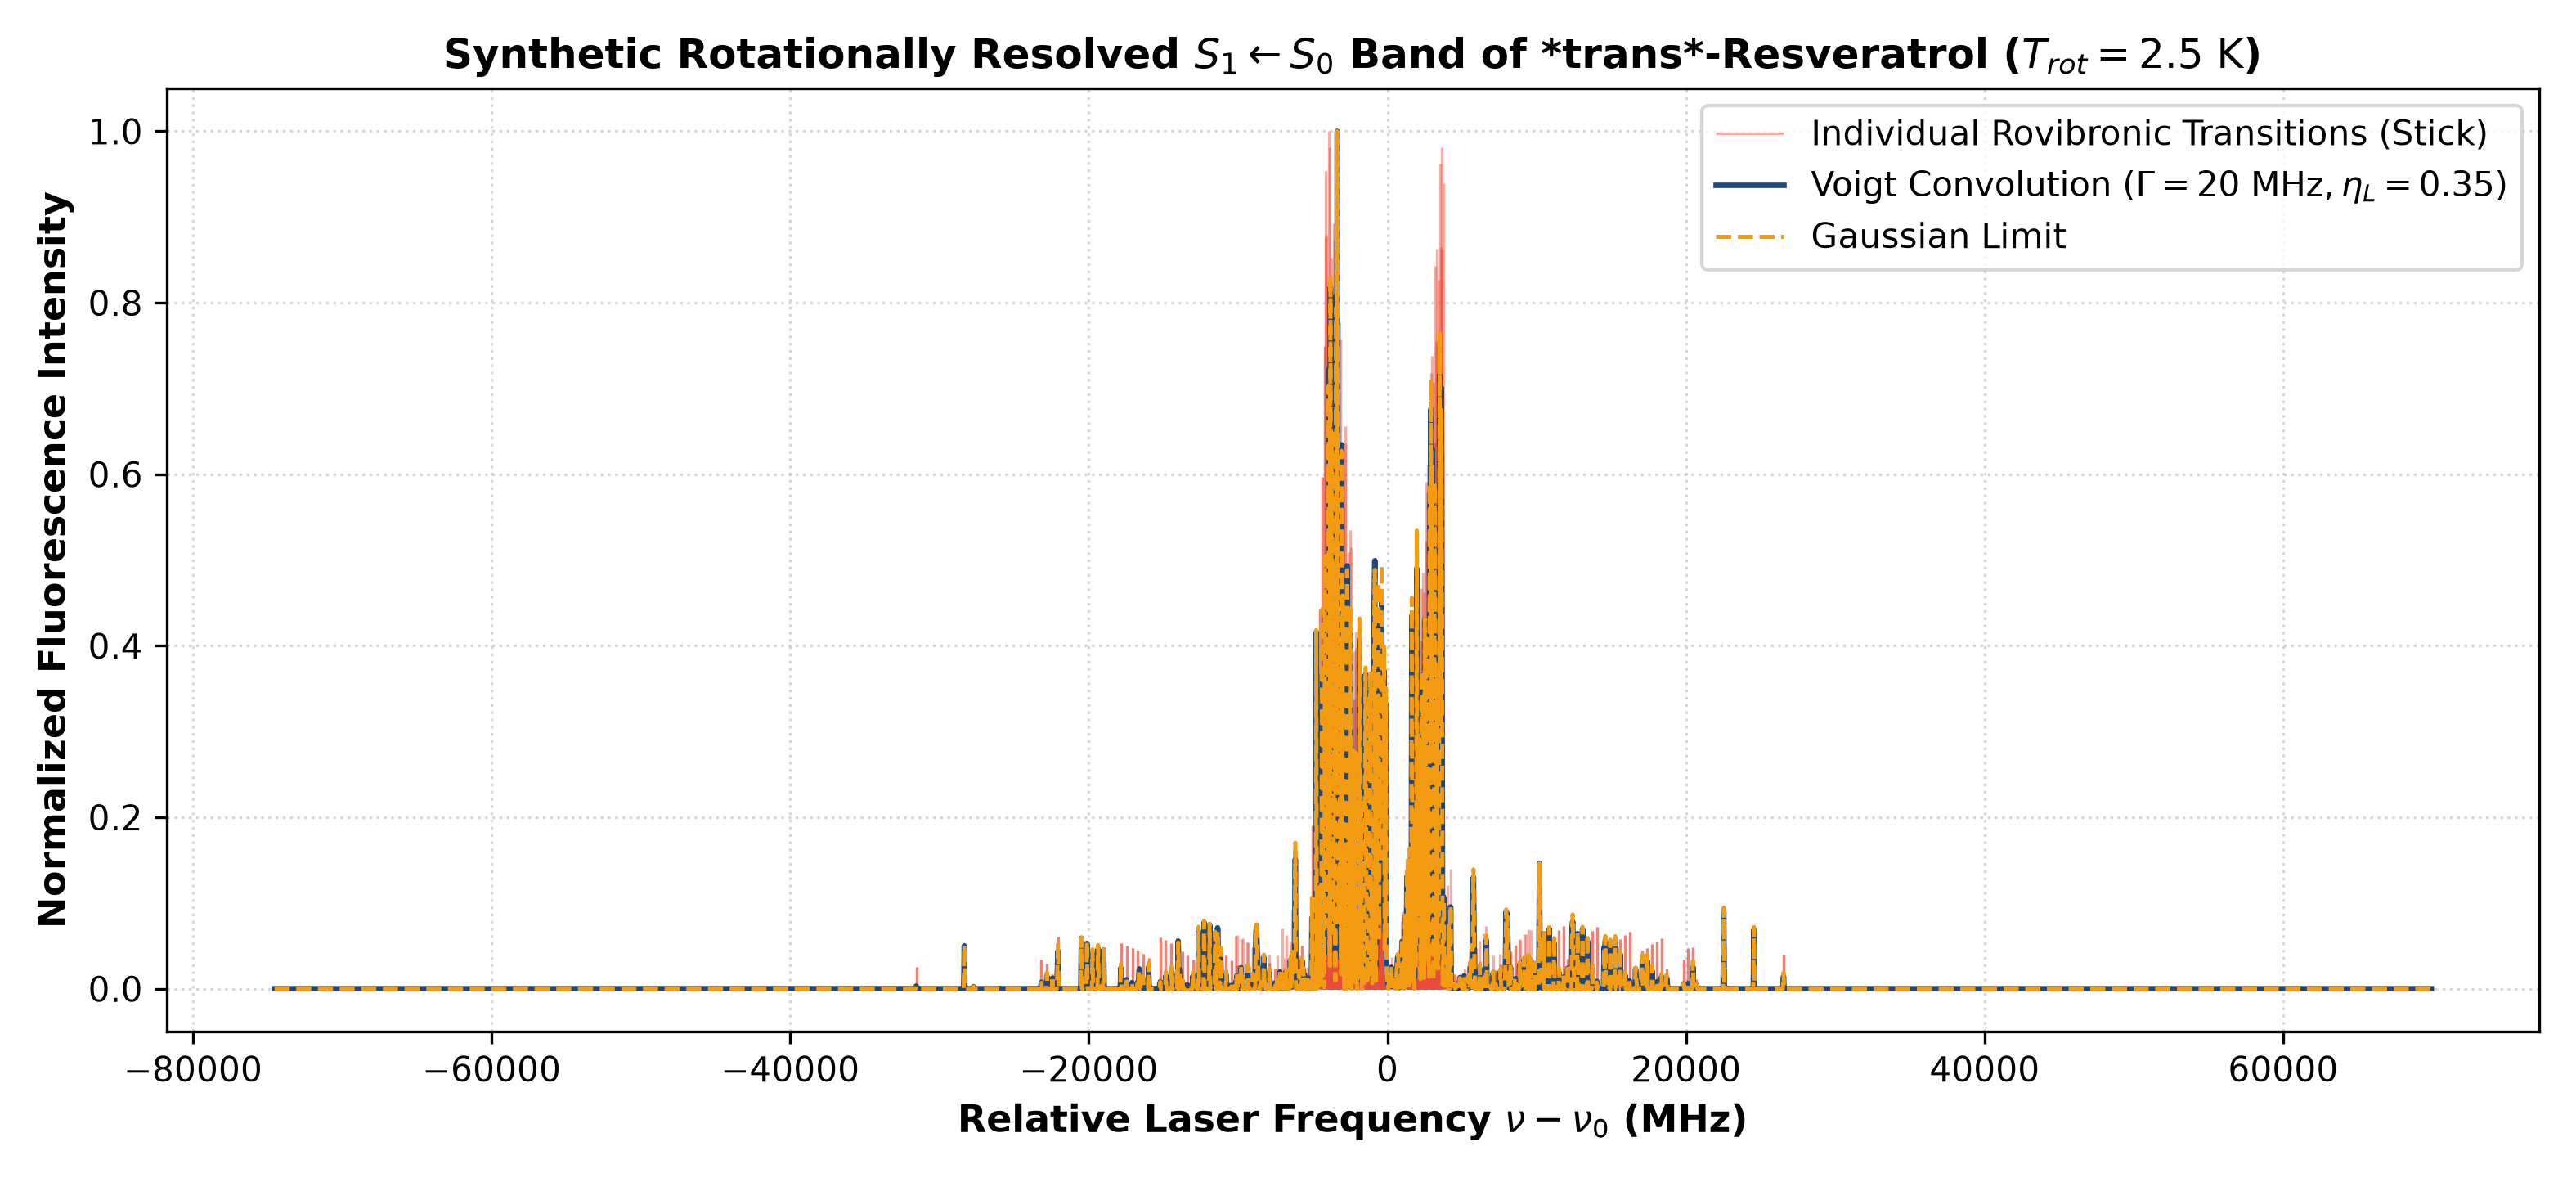
\includegraphics[width=\columnwidth]{figures/fig2_resveratrol_spectrum.png}
\caption{Synthetic rotationally resolved $S_1 \leftarrow S_0$ band contour of \textit{trans}-resveratrol at $T_{rot} = 2.5$~K. Over 2,400 transitions merge into a dense contour with a sharp $Q$-branch and resolved $P/R$ branch envelopes ($\text{FWHM} = 20$~MHz).}
\label{fig:spectrum_resv}
\end{figure}

\subsection{Rovibronic Spectrum of \textit{trans}-Resveratrol}
Figure~\ref{fig:spectrum_resv} displays the simulated $S_1 \leftarrow S_0$ origin band of Conformer~I at $T_{rot} = 2.5$~K. Over 2,400 individual transitions are populated up to $J = 11$. The spectrum is dominated by an intense central $Q$-branch ($\Delta J = 0$), flanked by symmetric $P$ ($\Delta J = -1$) and $R$ ($\Delta J = +1$) branches extending over $\pm 1500$~MHz. Unlike light rotors, individual lines coalesce into a smooth, highly congested band contour, illustrating why traditional line-assignment software fails.

\begin{figure}[t]
\centering
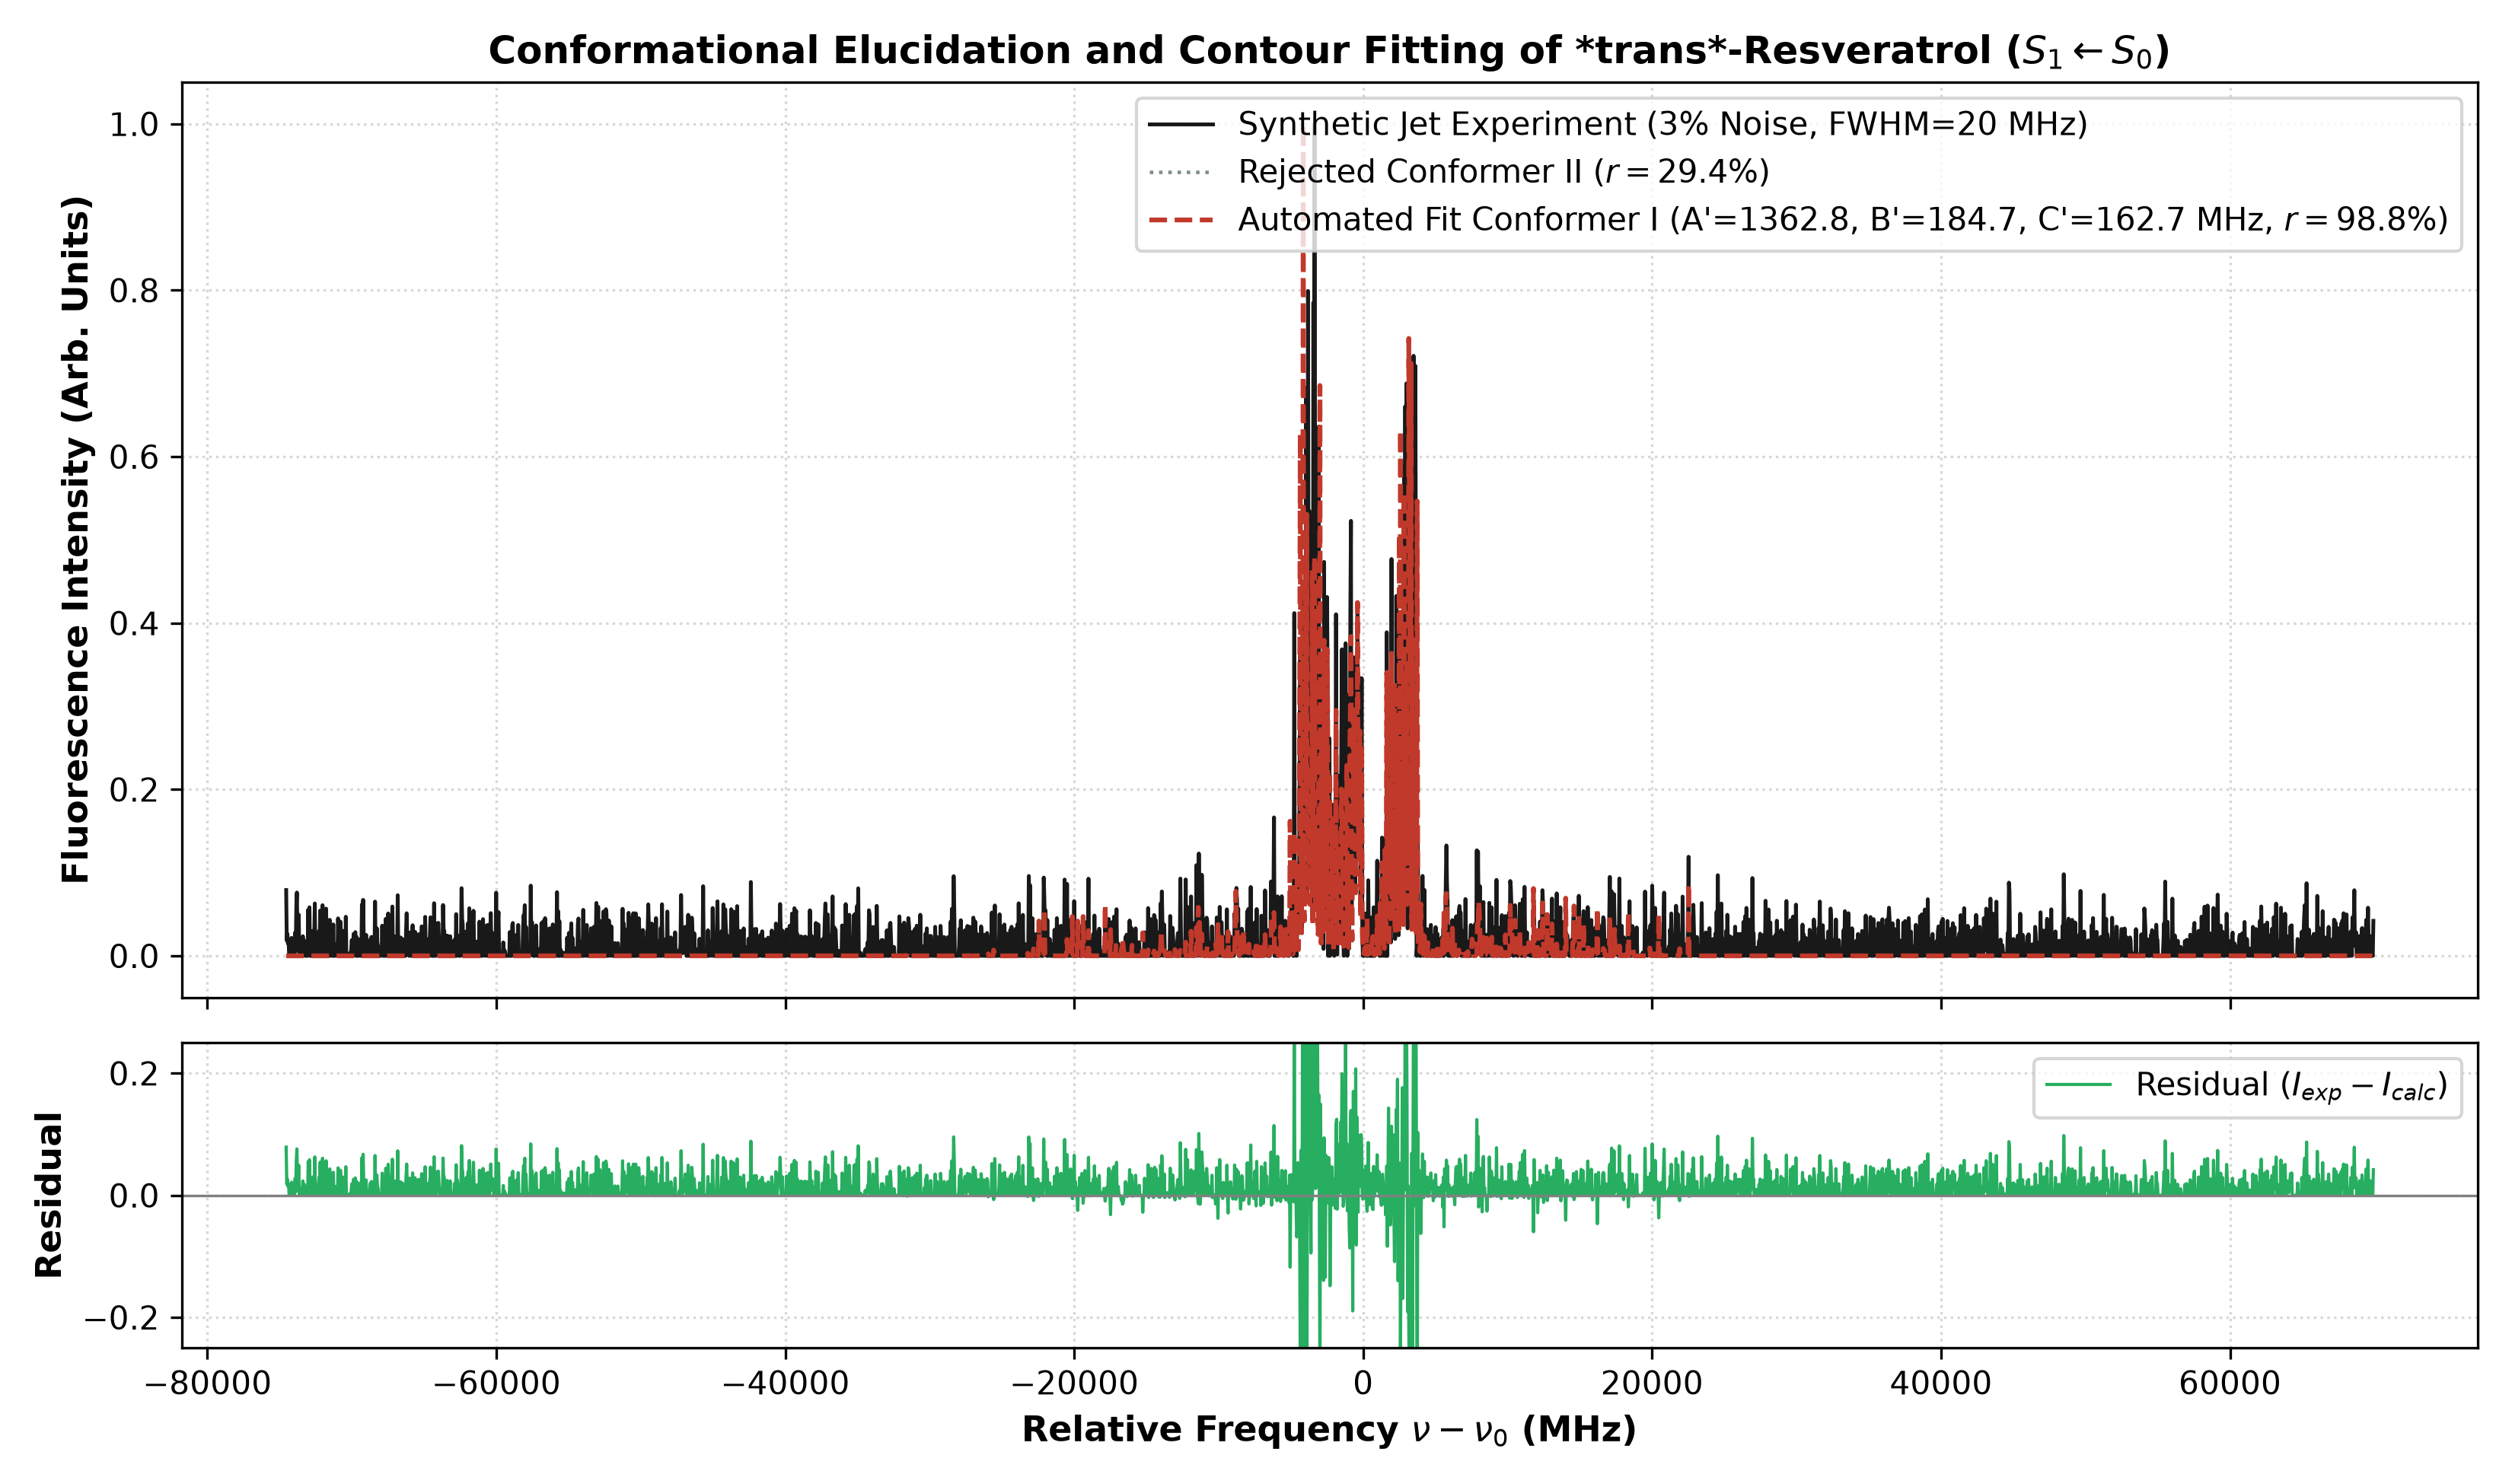
\includegraphics[width=\columnwidth]{figures/fig3_conformer_fit.png}
\caption{Automated conformational discrimination and contour fitting of \textit{trans}-resveratrol. Top: Synthetic jet data with 3\% noise (black), rejected Conformer~II trial ($r < 30\%$, gray dotted), and the converged Conformer~I fit ($r = 98.8\%$, red dashed). Bottom: Residual spectrum $(I_{exp} - I_{calc})$ bounded within the noise envelope.}
\label{fig:fit_resv}
\end{figure}

\subsection{Autonomous Conformational Discrimination \& Fitting}
To test the inverse problem solver, synthetic experimental data was corrupted with $3.0\%$ Gaussian noise. We formulated a two-stage hypothesis:
\begin{enumerate}
    \item \textit{Conformational Rejection:} Can the software differentiate between structural rotamers? Evaluating Conformer~II against the experimental profile yielded a normalized cross-correlation of $r < 30\%$ (Figure~\ref{fig:fit_resv}), leading to unambiguous rejection of the incorrect rotamer.
    \item \textit{Parameter Recovery for Conformer~I:} Starting from severely perturbed trial parameters ($A' = 1338.0$~MHz, $B' = 191.0$~MHz, $C' = 158.0$~MHz; shifted by up to 25~MHz), Differential Evolution converged autonomously to:
    \begin{itemize}
        \item $A'_{fit} = 1362.72$~MHz (True: $1362.80$~MHz, Residual: $0.08$~MHz)
        \item $B'_{fit} = 184.93$~MHz (True: $184.90$~MHz, Residual: $0.03$~MHz)
        \item $C'_{fit} = 162.78$~MHz (True: $162.80$~MHz, Residual: $0.02$~MHz)
        \item Band origin shift: $+0.04$~MHz.
    \end{itemize}
\end{enumerate}

The final correlation reached $98.8\%$, and the residual plot $(I_{exp} - I_{calc})$ shows complete convergence within the experimental noise threshold.

\section{Conclusions}
We have presented the application of \textbf{SpecWatson} to the complex natural polyphenol \textit{trans}-resveratrol. By combining Wang tridiagonal factorization with Differential Evolution contour fitting, the framework overcomes the severe spectral congestion characteristic of heavy biomolecules in supersonic molecular jets. The method provides sub-megahertz structural determination and robust conformational discrimination without requiring manual quantum number assignments. This establishes a powerful, automated platform for future high-resolution laser ablation studies of flexible natural products, antioxidants, and medicinal biomolecules.

\begin{acknowledgments}
The authors thank the Universidad de Guanajuato (Divisi\'on de Ciencias e Ingenier\'ias, Campus Le\'on) for institutional support and computational resources.
\end{acknowledgments}

\bibliography{references}

\end{document}
